	\documentclass[10pt,a4paper]{article}
	\usepackage[english]{babel}
	\usepackage[utf8]{inputenc}
	\usepackage{fancyhdr}
	\usepackage{hyperref}
	\usepackage{graphicx}
	\usepackage{subcaption}
	\usepackage{caption}
	\usepackage{cite}
	\usepackage{booktabs}
	\usepackage{wrapfig}
	\usepackage{float}
	\usepackage{xcolor}
	
	\restylefloat{table}

	\pagestyle{fancy}
	\fancyhf{}
	\rhead{26-April-2018}
	\lhead{Assignment 01}
	\rfoot{Page \thepage}

	\begin{document}
	\begin{titlepage}
	\centering

		{\scshape\LARGE Scientific Experimentation and Evaluation\par}

		{\scshape\Large Assignment: 02\par}

		\vfill

		\vfill
		{\Large\itshape Anees Khan (9030423)
			\\Debaraj Barua (9030412)\\
			Md Zahiduzzaman (9030432)
			\par}
		\vfill

		{\large 26-April-2018\par}
	\end{titlepage}
	\tableofcontents
	\listoffigures	
	\listoftables
	\newpage
	\section{Relevant Aspects of Experiment}
	\subsection{Design of Robot}
		\begin{itemize}
			\item The robot has been designed with three wheels.
			\item Two of these are driving wheels and are connected to the motors, thus enabling a differential drive systems; and \textcolor{blue}{the third is a caster wheel at the back}.
			\item Wheels are oriented as shown in the \textcolor{blue}{images below}.
			\begin{figure}[H]
				\begin{subfigure}{0.5\textwidth}
					\centering
					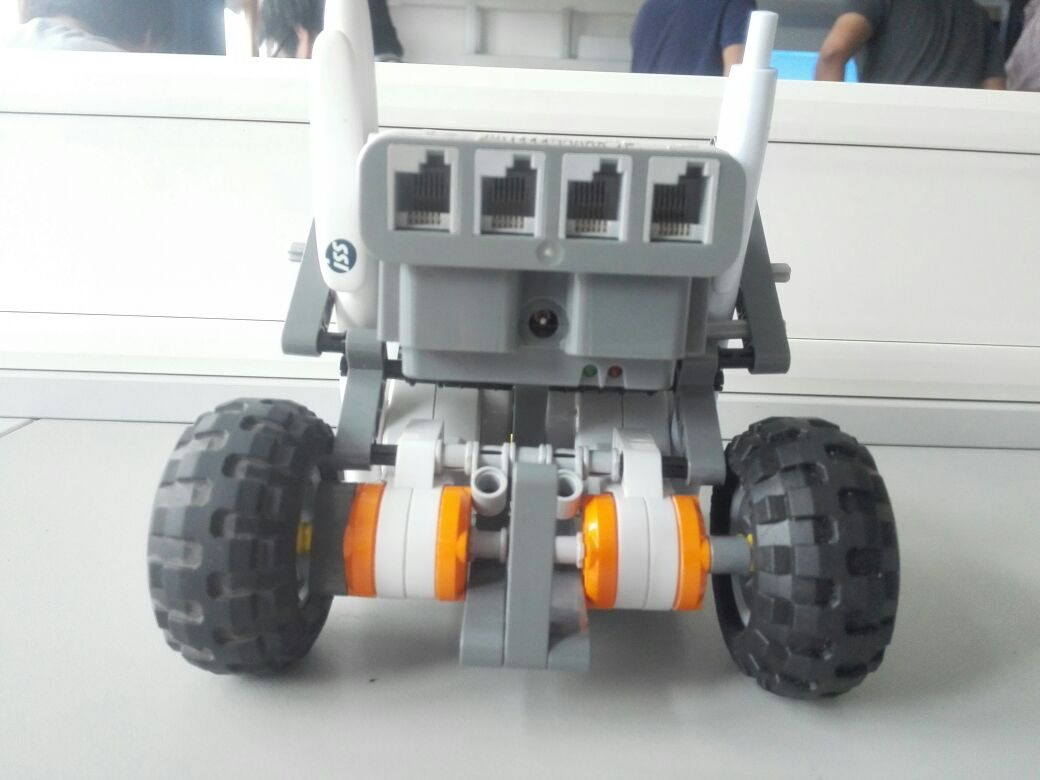
\includegraphics[width=0.8\linewidth]{img/front.jpeg}
					\caption{Front View}
					\label{fig:fview}
				\end{subfigure}%
				\begin{subfigure}{0.5\textwidth}
					\centering
					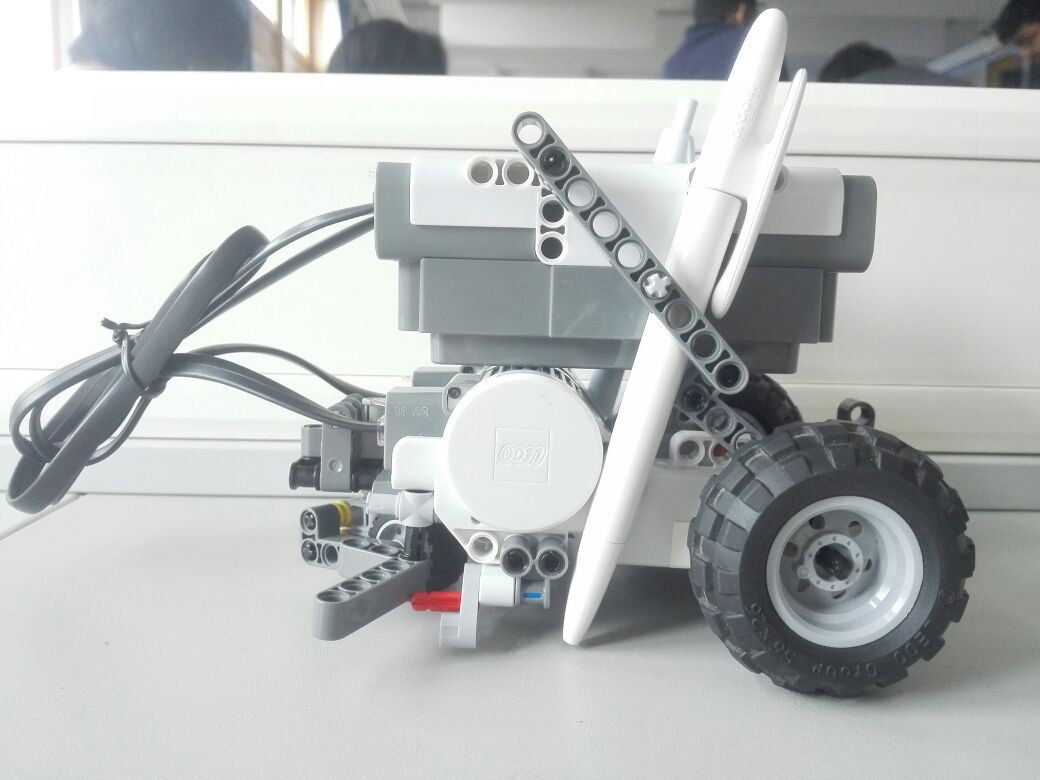
\includegraphics[width=0.8\linewidth]{img/right.jpeg}
					\caption{Right View}
					\label{fig:rview}
				\end{subfigure}
				\begin{subfigure}{0.5\textwidth}
					\centering
					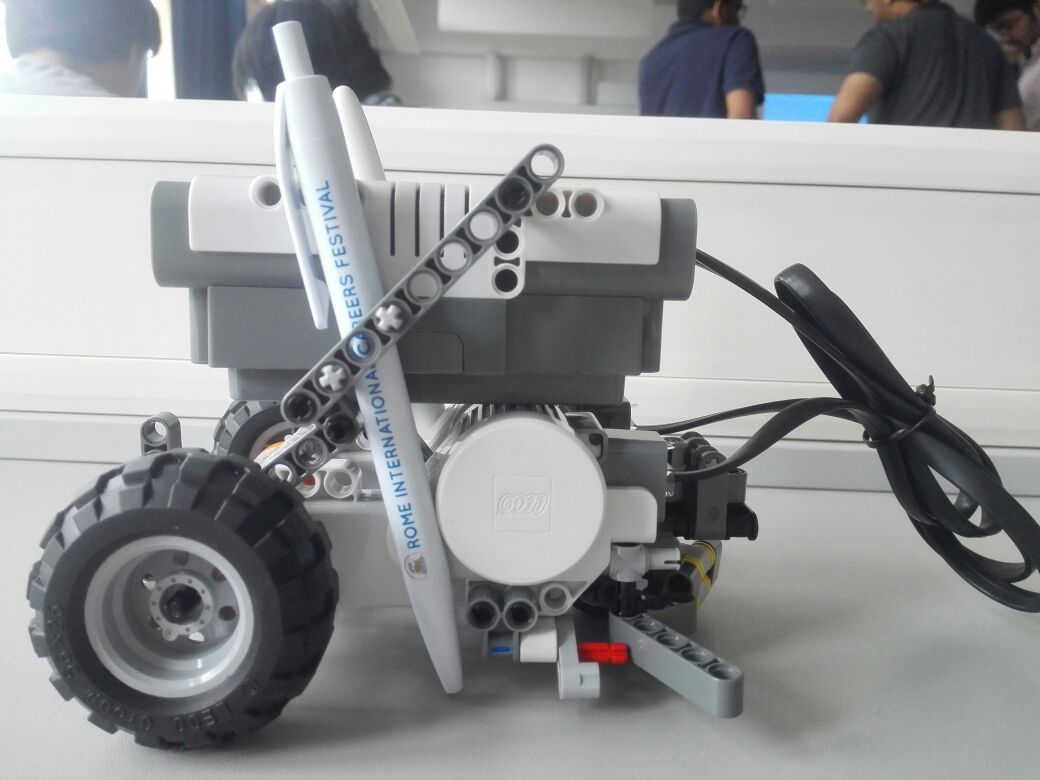
\includegraphics[width=0.8\linewidth]{img/left.jpeg}
					\caption{Left View}
					\label{fig:lview}
				\end{subfigure}
				\begin{subfigure}{0.5\textwidth}
					\centering
					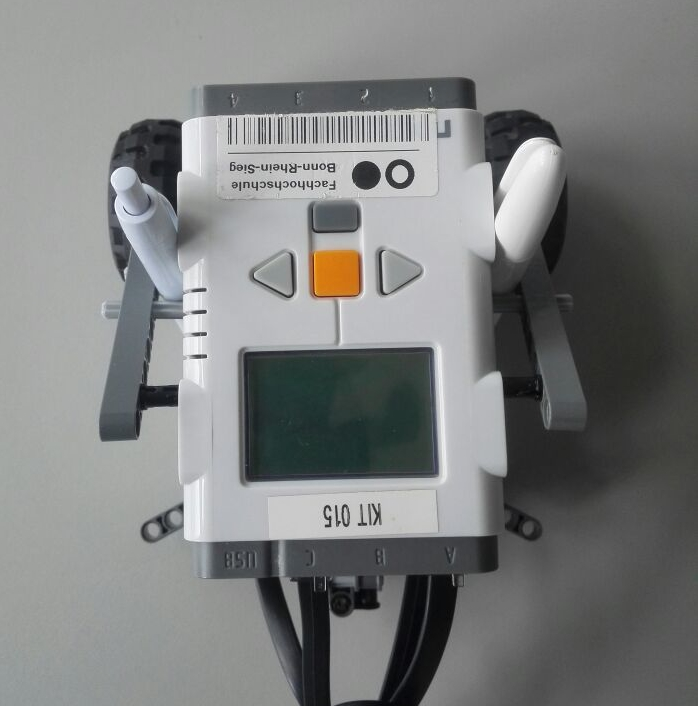
\includegraphics[width=0.8\linewidth]{img/top.jpeg}
					\caption{Top View}
					\label{fig:tview}
				\end{subfigure}
				\begin{subfigure}{0.5\textwidth}
					\centering
					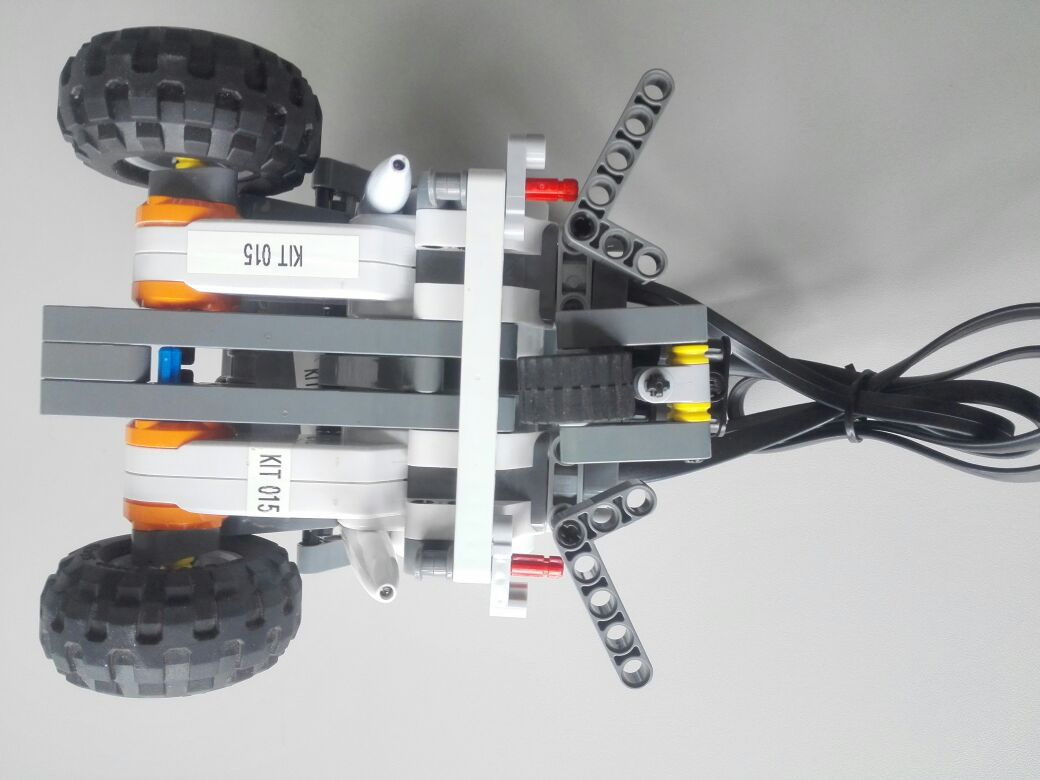
\includegraphics[width=0.8\linewidth]{img/bottom.jpeg}
					\caption{Bottom View}
					\label{fig:bottomview}
				\end{subfigure}
				\caption{Robot Design}
				\label{fig:Robotfig}
			\end{figure}
			\item \textcolor{blue}{In addition, as shown above in the bottom view, it is ensured that the caster wheel does not rotate 360$^\circ$}.
		\end{itemize}
		
	\subsection{Transformations}\textcolor{red}{
			- Distance from pen axis to wheel axis = 5 cm \\
			- Distance between the mid points of the two wheels (track width) = 11.5 cm \\
			- WRITE FORMULA
			}
	\subsection{Measurement of Start and Stop Positions}
		\subsubsection{Measurement Instruments}\textcolor{blue}{
			\begin{itemize}
				\item Distance:
				\begin{itemize}
					\item We use a scale ruler to measure the distances.
					\item In addition, we also utilize the grids on the paper which acts as our workspace and world coordinate systems.
					\item Instrument Details:
					\begin{itemize}
						\item 1 square of the grid paper equals $2.5 \times 2.5$ cm
						\item The precision of the scale used is 1 mm.
					\end{itemize}
				\end{itemize}
				\item Angle:
				\begin{itemize}
					\item A protractor is used as a measuring instrument for the angles.
					\item Instrument Details:
					\begin{itemize}
						\item Precision of the protractor used is 1$^\circ$.
					\end{itemize}
				\end{itemize}
			\end{itemize}
		}
		\subsubsection{Measurement Procedure} \textcolor{blue}{
		\begin{itemize}
			\item Two pens will be fixed near the two driving wheels.
			\item The starting position is where the two pens meets the x -axis, with the left pen lying on the origin (right pen at a distance of  8.3 cm from the origin).			
			\begin{figure}[h]
				\centering
				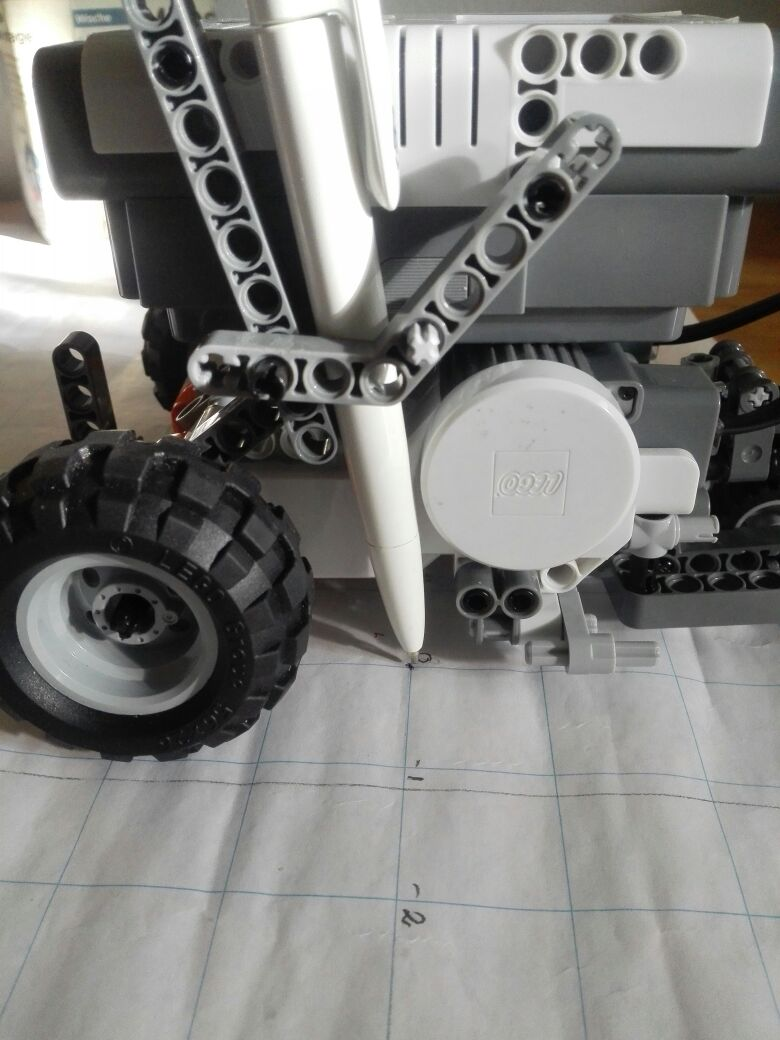
\includegraphics[width=0.4\linewidth]{img/starting-pt.jpeg}
				\caption{Staring Position}
				\label{fig:startingView}
			\end{figure}
			\item To measure the orientation of robot, the two points from these pens will be joined by drawing a line, which will be used to mark the pose of robot, with respect to the coordinate system defined.
			\item For each run, at the initial condition, it is ensured that orientation of rear caster wheel axle is parallel to the driving wheel axis.
			\item Measuring Position:
				\begin{itemize}
					\item To get the position of the robot, we measure the distance of the two points from X and Y axis using a scale ruler.
					\item These two readings are put in the transformation equation described above to get the actual position of the robot.
				\end{itemize}
			\item Measuring Angles:
				\begin{itemize}
					\item The angular pose of the robot is the angle the X-axis makes with the normal to the line joining the two points.
					\item This angle is equal to the angle Y-axis makes with the line joining the two points. This can be verified using basic geometry, as shown in the image below.
					\begin{figure}[h]
						\centering
						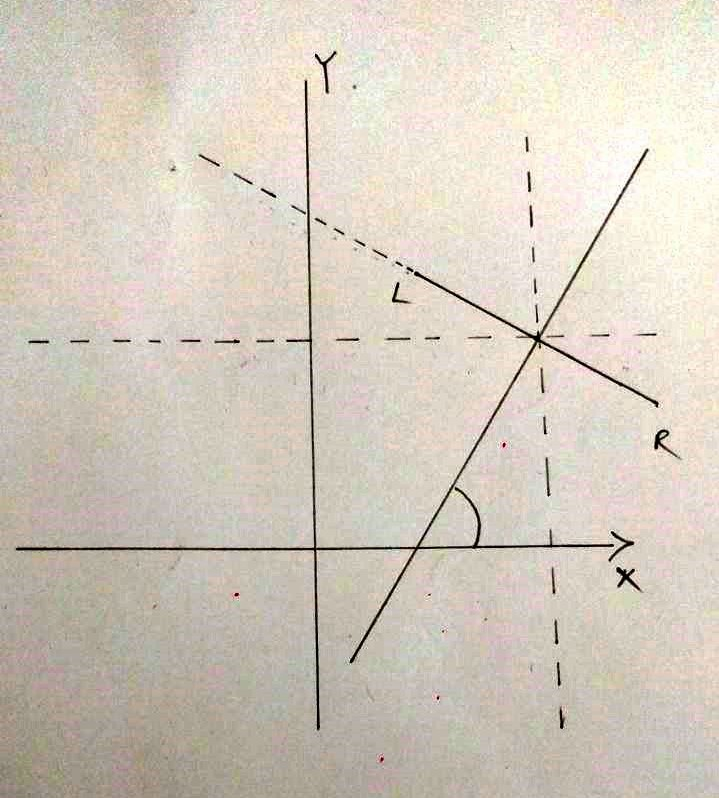
\includegraphics[width=0.4\linewidth]{img/angles.jpeg}
						\caption{Measurement of angles}
						\label{fig:angGeometry}
					\end{figure}
					\item We now measure the angle using a protractor.
				\end{itemize}
		\end{itemize}
		}
	\subsection{Parameters used to drive the robot}
		\begin{itemize}
			\item Constant angular and translational speed for a fixed time period to describe an arc to left.
			\item Constant translational speed and no angular speed for a fixed time period to describe a straight line.
			\item Constant angular and translational speed for a fixed time period to describe an arc to right.
		\end{itemize}
	\subsection{Program used to drive the robot}
		\begin{itemize}
			\item Using the Lego Mindstorms NXT 2.0 software, we created the scenarios for three run sequences.
			\item Straight Line:
				\begin{itemize}
					\item Power: 50\%
					\item Duration: 3 Seconds
					\item Steering Angle: 0 degrees
				\end{itemize}
			\item Left Arc:
				\begin{itemize}
					\item Power: 50\%
					\item Duration: 3 Seconds
					\item Steering Angle: -45 degrees
				\end{itemize}
			\item Right Arc:
				\begin{itemize}
					\item Power: 50\%
					\item Duration: 3 Seconds
					\item Steering Angle: 45 degrees
				\end{itemize}		
			\item The power percentage to wheel rpm has been calculated on the basis of readings found in \cite{motorInternals}. It is observed that in the unloaded condition, 50\% power results to around 80 rpm
			\item Diameter of wheels: 5.7 cm
		\end{itemize}
	\subsection{Expected Problems and Performance}
		\begin{itemize}
			\item Axis connecting the two pens might not be parallel to the wheel axle.
			\item Start position of each run may not be exactly similar owing to inaccurate positioning of the robot, this will result in lower precision.
			\item Pens may slip of move during the run, as such may not result in accurate positions, thus affecting the precision of our readings.
			\item The constant angular and translational speeds that we assume, may be inaccurate. The actual speed may differ and thus our estimate from the time will be inaccurate.
			\item The initial acceleration and final deceleration of the robot has not been considered in the experiments, resulting in low accuracy.
			\item In addition of the two previous points, slippage in the wheels and motors will also affect the accuracy of readings.
			\item The driven wheel will also result in the bot to drift and also decrease the distance it reaches.
			\item In addition, the calculation of expected position in each case is based on percentage of power applied to the motor and duration for which it is applied. However, this may result in an overestimate because of the following:
				\begin{itemize}
					\item Actual power output may depend on the charge in batteries and the efficiency of motor.
					\item Speed of the robot is calculated on the basis of this power output and the load on wheels, for calculation, we have approximated the motor rpm to a no-load condition. This is not true in the actual experiment.
				\end{itemize} 
		\end{itemize}
	\section{Observations and Data}
		\subsection{Readings}
		\begin{table}[H]
			\centering
			\begin{tabular}{lrrrrr}
				\toprule
				{} &  X\_L(cm) &  Y\_L(cm) &  X\_R(cm) &  Y\_R(cm) &  Angle(degrees) \\
				\midrule
				0 &        0 &        0 &      8.3 &        0 &              90 \\
				\bottomrule
			\end{tabular}
			\caption{Intial Position}
		\end{table}
		\begin{table}[H]
			\centering
			\begin{table}[H]
\centering
\caption{Final Pose along straight direction}
\label{straight}
\begin{tabular}{|l|c|c|c|}
	\hline
	\multicolumn{1}{|c|}{Object Type} & X (cm) & Y (cm) &  $\theta$ (radians)   \\ \hline
	Small                             & -90.34 & -75.31 & 1.40				    \\ %\hline
	Medium                            & -87.85 & -71.63 & 1.48				    \\ %\hline
	Large                             & -84.00 & -67.94 & 1.39    				\\ \hline
	Combined                          & -87.40 & -71.63 & 1.42				    \\ \hline
\end{tabular}
\end{table}

			\caption{Straight Line Position}
		\end{table}
		\begin{table}[H]
			\centering
			\input{leftArc}
			\caption{Left Arc Position}
		\end{table}
		\begin{table}[H]
			\centering
			\input{rightArc}
			\caption{Right Arc Position}
		\end{table}
		Detailed data is available in the file "Assignment01\_data.ods"
	 \subsection{Visualization}
		 \begin{figure}[H]
		 	\centering
		 	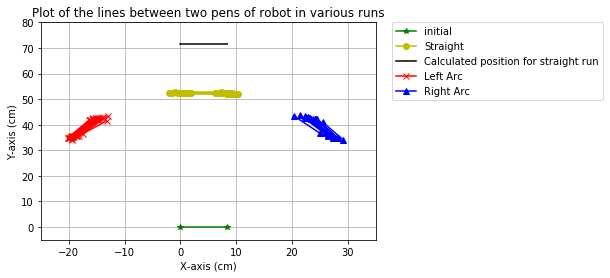
\includegraphics[scale=0.5]{line_plot.png}
		 	\caption{Plot of the lines between two pens of robot in various runs}
		 \end{figure}
		 \begin{figure}[H]
		 	\centering
		 	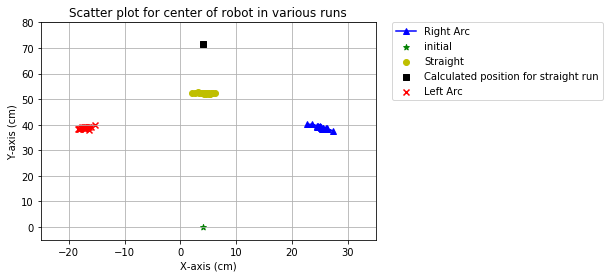
\includegraphics[scale=0.5]{scatter_plot.png}
		 	\caption{Scatter plot for center of robot in various runs}
		 \end{figure}
	 All the plots and code is available in the file "SEE\_Experiment01\_plots.ipynb"		
	\section{Results}
			\begin{figure}[h]
				\centering
				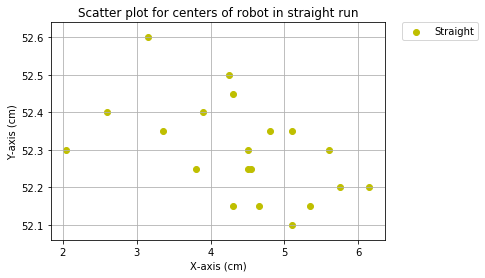
\includegraphics[width=0.7\textwidth]{scatter_plot_st.png}
				\caption{Scatter plot for centers of robot in Straight run}
			\end{figure}
			\begin{figure}[h]
				\centering
				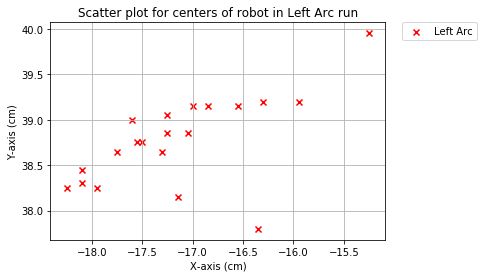
\includegraphics[width=0.7\textwidth]{scatter_plot_lt.png}
				\caption{Scatter plot for centers of robot in Left Arc run}
			\end{figure}
			\begin{figure}[h]
				\centering
				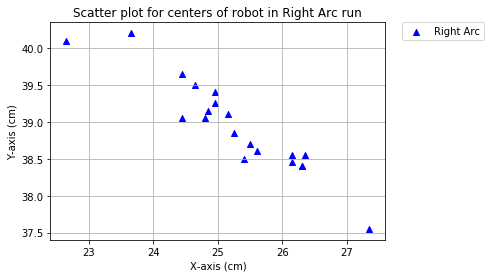
\includegraphics[width=0.7\textwidth]{scatter_plot_rt.png}
				\caption{Scatter plot for centers of robot in Right Arc run}
			\end{figure}
	\begin{itemize}
		\item Straight Run:		
			\begin{itemize}
				\item Mean X value: 52.3 cm
				\item Mean Y value: 4.4 cm
				\item Mean Angular value: 88.7 degrees
				\item Standard Deviation in X value: 1.0 cm
				\item Standard Deviation in Y value: 0.1 cm
				\item Standard Deviation in Angular value: 1.0 degrees
				\item Accuracy: 73 \%
			\end{itemize}
		\item Left Arc:
			\begin{itemize}
				\item Mean X value: -17.2 cm
				\item Mean Y value: 38.8 cm
				\item Mean Angular value: 145.6 degrees
				\item Standard Deviation in X value: 0.8 cm
				\item Standard Deviation in Y value: 0.5 cm
				\item Standard Deviation in Angular value: 2.3 degrees
			\end{itemize}
		\item Right Arc	:
			\begin{itemize}
				\item Mean X value: 25.2 cm
				\item Mean Y value: 39.0 cm
				\item Mean Angular value: 33.7 degrees
				\item Standard Deviation in X value: 1.0 cm
				\item Standard Deviation in Y value: 0.6 cm
				\item Standard Deviation in Angular value: 2.3 degrees
			\end{itemize}	
	\end{itemize}
	The details of calculations of these values is available in the file "SEE\_Experiment01\_plots.ipynb"

	\bibliography{references.bib}
	\bibliographystyle{plain}
	\end{document}
